\documentclass[10pt,letterpaper,twocolumn]{article}

\usepackage{iclr2026_conference}

\usepackage[T1]{fontenc}
\usepackage[utf8]{inputenc}
\usepackage{amsmath}
\usepackage{amssymb}
\usepackage{booktabs}
\usepackage{multirow}
\usepackage{url}
% Two 245bp columns of Times leave little room for a bad line break, and the
% draft had several paragraphs stretched past readability. Expansion recovers
% them. Protrusion is switched off deliberately: it hangs punctuation about
% 1bp past the column edge, which is good typography but puts glyphs outside
% the frame the venue specifies, and verify_format.py reads it as a wider
% column.
\usepackage[protrusion=false]{microtype}
\usepackage[numbers,sort&compress]{natbib}
\usepackage[hidelinks]{hyperref}

\newcommand{\vhat}{\hat{\mathbf{v}}}
\newcommand{\yv}{\mathbf{y}}
\newcommand{\zv}{\mathbf{z}}

\title{Does a Head Attend to Its Own Value?\\
Null-Controlled Tests of Self-Attention Redundancy}

\author{Anonymous Author\textsuperscript{1}}
\iclraffiliation{\afmark{1}Anonymous Institution}
\iclremail{anon@example.invalid}

\begin{document}

\twocolumn[
\maketitle
\begin{iclrabstract}
A recurring informal claim about transformer language models is that each
attention head partly re-reads the value vector it has itself written, and
that this self-directed component is redundant and can be removed at no cost.
The claim is easy to state and hard to test, because the obvious test---delete
the component and see whether loss moves---has no reference point: almost any
rank-one edit to a residual stream moves loss a little. We give the claim a
falsifiable form by pairing every intervention with a matched null, and by
first asking whether the effect is resolvable at all. Our protocol has three
stages: a split-half reliability check that bounds the largest correlation the
measurement could possibly show, an anisotropy null that compares a head's
self-directed cosine against a partner position drawn from the causally
attendable set, and a matched intervention that compares removing the
self-directed direction against removing an arbitrary rank-one direction of the
same norm. Across twelve pretrained models we find the structural statistic is
reliable in only one of three models tested at depth, and that the correlation
between the structural statistic and the measured behavioural effect is weak
even after disattenuation. In an eight-seed paired factorial trained from
scratch at $4.0\times10^{8}$ tokens per run, the pre-registered
arbitrary-direction control is indistinguishable from baseline ($+0.00106$
nats, $p=0.197$), while removing the self-directed direction is reliably
harmful ($-0.00292$ nats, Holm-corrected $p=0.0023$). The self-directed
component is therefore \emph{not} redundant, and the structural statistic that
motivated the claim does not predict the behavioural effect.
\end{iclrabstract}
\vspace{6pt}
]

\section{Introduction}

Multi-head self-attention \citep{vaswani2017attention} writes a value vector
for every position and every head, and then reads a convex combination of
those vectors back out. Because a causal mask admits the diagonal, the
combination at position $i$ includes the value vector written at position $i$
by the same head. This has produced a persistent informal claim: the
self-directed portion of the read is a self-loop that carries no information
the residual stream does not already hold, so it is redundant and could be
removed without cost. The claim appears in discussions of head pruning
\citep{michel2019sixteen,voita2019analyzing} and of attention as a set of
composable circuits \citep{elhage2021mathematical}, usually as an aside rather
than as a measured result.

The claim is awkward to test for a reason that is easy to miss. The natural
experiment---project the self-directed direction out of a head's output and
measure the change in language-modelling loss---produces a number, and that
number is almost never zero. Residual streams are anisotropic
\citep{ethayarajh2019contextual}; removing any rank-one direction of comparable
norm perturbs the model. Without a reference, a small non-zero $\Delta$
supports whichever reading the analyst brought to it. A related problem sits
one level up: correlating a structural statistic (how self-directed a head is)
against a behavioural one (how much removing it hurts) is only informative if
both are measured reliably enough for a correlation to exist. Reported
correlations near zero are routinely read as decoupling when they are equally
consistent with a measurement too noisy to resolve anything.

We therefore treat ``the self-directed component is redundant'' as a hypothesis
that needs a null, and we ask three questions in a fixed order.

\paragraph{Check 0: is the effect resolvable?} Before any correlation is
interpreted, we estimate the split-half reliability $r_\Delta$ of the
behavioural effect and $r_{\text{stat}}$ of the structural statistic. Their
geometric mean $\sqrt{r_\Delta r_{\text{stat}}}$ bounds the largest correlation
that could be observed even if the underlying quantities were identical. If
that ceiling is below $0.3$ we report the measurement as unresolvable rather
than reporting a null result.

\paragraph{Check 1: is the self-directed cosine anisotropy?} We compare
$\cos(\yv_i, \mathbf{v}_i)$ against the same cosine computed with a null
partner drawn uniformly from the positions the head could causally have
attended to. A self-directed read that is merely the ambient geometry of the
space shows no gap.

\paragraph{Check 2: does removal hurt more than a matched edit?} We compare
removing the self-directed direction against removing an arbitrary rank-one
direction of matched norm, as paired arms of the same training run, with the
arbitrary direction pre-registered as the primary endpoint.

\paragraph{Contributions.}
\begin{itemize}\itemsep2pt \parsep0pt \topsep2pt
\item A three-stage protocol that makes ``this component is redundant''
falsifiable, with the resolvability check placed before rather than after the
correlation is interpreted (Section~\ref{sec:method}).
\item A measured reconstruction gate that verifies the attention decomposition
is layout-correct before any intervention is trusted; the threshold is derived
from the observed separation between the correct layout and four deliberately
broken ones, not assumed (Section~\ref{sec:gate}).
\item An eight-seed paired factorial at $4.0\times10^{8}$ tokens per run
showing that the pre-registered arbitrary-direction control is
indistinguishable from baseline while self-directed removal is reliably
harmful, which falsifies the redundancy claim in the direction opposite to the
one usually assumed (Section~\ref{sec:paired}).
\item Reliability and disattenuated correlation estimates across twelve
pretrained models showing that the structural statistic resolves in one of
three models tested at depth, and predicts the behavioural effect weakly even
there (Section~\ref{sec:a2}).
\end{itemize}

\section{Related Work}

\paragraph{Head importance and pruning.} \citet{michel2019sixteen} and
\citet{voita2019analyzing} both establish that a large fraction of heads can be
removed with small loss penalties, and both measure importance by ablation.
Neither pairs the ablation with a matched control edit, so the reported
penalties conflate the specific structure removed with the generic cost of
perturbing the residual stream. Our Check~2 is that missing control.

\paragraph{Circuit-level accounts.} \citet{elhage2021mathematical} decompose
attention into $QK$ and $OV$ circuits and treat the diagonal of the attention
pattern as one term among many. The self-directed read we study is exactly the
diagonal contribution to the $OV$ circuit, isolated and intervened on rather
than described.

\paragraph{Representation geometry.} \citet{ethayarajh2019contextual} show that
contextual representations occupy a narrow cone, which is the reason a raw
self-cosine is uninformative and the reason Check~1 needs a matched null
partner drawn from the causally attendable set rather than from the whole
range of positions.

\paragraph{Grouped-query attention.} \citet{ainslie2023gqa} share key and value
projections across groups of query heads. This gives a natural test of whether
the self-directed statistic tracks parameter sharing, which we report in
Section~\ref{sec:gqa}.

\section{Method}
\label{sec:method}

\subsection{The intervention}

Let head $h$ at layer $\ell$ produce output $\yv_i \in \mathbb{R}^{d_h}$ at
position $i$, and let $\mathbf{v}_i$ be the value vector that same head writes
at $i$. Write $\vhat_i = \mathbf{v}_i / \lVert \mathbf{v}_i \rVert$. The
self-directed removal, which we call XSA, replaces the head output with
%
\begin{equation}
\zv_i \;=\; \yv_i \;-\; \tanh(\alpha)\,\langle \yv_i, \vhat_i\rangle\,\vhat_i ,
\label{eq:xsa}
\end{equation}
%
where $\alpha$ is a per-head gate. For a frozen pretrained model the gate is
held fully open, $\tanh(\alpha)=1$, so the projection onto $\vhat_i$ is removed
exactly and the measurement is of the component itself rather than of what a
model would choose to do with it. In the trained factorial the gate is learned,
which lets the model discard the intervention if the component really is
redundant; Section~\ref{sec:paired} reports what it does instead.
Equation~\ref{eq:xsa} is a rank-one edit applied per head, per position, before
the output projection.

The matched control, which we call \textsc{random}, applies the identical edit
with $\vhat_i$ replaced by a direction drawn uniformly on the unit sphere and
resampled per position, so the two arms differ only in \emph{which} rank-one
direction is removed and not in how much norm is removed in expectation. Two
further arms are used as sanity anchors: \textsc{meanval}, which removes the
direction of the batch-mean value vector, and \textsc{diagmask}, which zeroes
the attention diagonal before the softmax so the row renormalises over the
remaining keys.

\subsection{Check 0: resolvability}

Split the evaluation corpus into halves $A$ and $B$. For every head compute the
behavioural effect $\Delta$ on each half and the structural statistic on each
half, and take Spearman correlations across heads to obtain the split-half
reliabilities $r_\Delta$ and $r_{\text{stat}}$, each corrected to full length by
Spearman--Brown. The largest correlation observable between the two quantities
is then
%
\begin{equation}
\rho_{\max} \;=\; \sqrt{r_\Delta \, r_{\text{stat}}},
\qquad
\rho_{\text{disatt}} \;=\; \rho_{\text{raw}} / \rho_{\max}.
\label{eq:ceiling}
\end{equation}
%
We declare the measurement \emph{reliable} at $r_\Delta \ge 0.6$,
\emph{attenuated} at $0.3 \le r_\Delta < 0.6$, and \emph{unresolvable} below
$0.3$. Under the last verdict we report no correlation at all, because a raw
$\rho$ near zero would be indistinguishable from noise.

Two details matter and are easy to get wrong. First, $r_{\text{stat}}$ must be
computed per statistic: reusing the reliability of one statistic to
disattenuate another inflates the result. Second, the half-split statistic must
be paired against a half-split effect, not against the two-half effect, or the
denominator and numerator are estimated at different sample sizes.

\subsection{Check 1: the anisotropy null}

For each head and position, $\cos(\yv_i, \mathbf{v}_i)$ is compared against
$\cos(\yv_i, \mathbf{v}_j)$ with $j$ drawn uniformly from
$\{1,\dots,i\}$, the set of positions the head could causally have attended to.
The reported statistic, \emph{excess}, is the paired difference. Confidence
intervals use a cluster bootstrap over layers rather than a row bootstrap over
heads: heads within a layer share an input and are not independent, and a row
bootstrap treats them as if they were.

\subsection{Check 2: matched intervention}
\label{sec:check2}

Check~2 is run as a paired factorial over seeds. For each seed, all arms train
from an identical initialisation on an identical token stream, so the paired
difference removes seed variance. The pre-registered primary endpoint is
\textsc{random} versus baseline: if an arbitrary rank-one removal is already
harmful, no conclusion about the self-directed one is available. The
self-directed comparison is a secondary endpoint and is Holm-corrected
\citep{holm1979simple} across secondaries only.

The minimum detectable effect at $80\%$ power and $\alpha = 0.05$ is
%
\begin{equation}
\text{MDE} \;=\; 2.9\,\sigma_{\text{paired}} \big/ \sqrt{n},
\label{eq:mde}
\end{equation}
%
which we report as a \emph{realised measurement} computed from the observed
$\sigma_{\text{paired}}$, and distinguish throughout from the planning forecast
made before the runs were executed.

\subsection{The reconstruction gate}
\label{sec:gate}

An intervention on $\yv_i$ is only meaningful if $\yv_i$ has been decomposed
correctly, and head-dimension layout errors are silent: a transposed or rolled
head axis still produces a tensor of the right shape and a plausible loss. We
therefore rebuild $\yv = A\,\mathrm{expand\_kv}(V)$ from the captured attention
matrix and value tensor and gate on the relative Frobenius error.

The threshold is measured rather than assumed. Under the correct layout the
error is $2.0\times10^{-4}$; under four deliberately broken layouts (heads
reversed, head axis rolled, transpose omitted, key--value expansion skipped) it
is $1.39$ to $1.50$. Any threshold in that gap separates them, and we take
$10^{-2}$, which is two orders of magnitude above the correct layout and two
below the nearest failure. The gate fails closed on non-finite values, since a
comparison against \texttt{NaN} is false and an ungated \texttt{NaN} would pass
silently.

\section{Experimental Setup}

\paragraph{Frozen-model measurements.} Checks 0 and 1 are run on twelve
pretrained models spanning $70$M to $6.9$B parameters, including the GPT-2
family \citep{radford2019language}, the Pythia suite
\citep{biderman2023pythia}, and grouped-query models. Every model is pinned by
revision hash. Documents are truncated to a fixed sequence length of $128$
tokens; documents shorter than that are dropped rather than padded, because
Check~1's null partner set is length-dependent and a drifting sequence length
would change the statistic between runs.

\paragraph{Trained factorial.} Check~2 trains a small decoder-only model from
scratch on eight seeds (7, 42, 99, 512, 1337, 2024, 8191, 31337) under three
arms (\textsc{baseline}, \textsc{xsa}, \textsc{random}), giving 24 cells.
Each cell sees $399\,900\,672$ tokens, a batch-aligned floor derived from the
budget rather than a round number: the token count is rounded down to a
multiple of the per-step token count so that no cell stops mid-batch. Iteration
is seed-major, so that if the compute budget is exhausted the result is a whole
number of complete paired seeds rather than a scatter of orphaned cells.

\paragraph{Budget.} All runs fit a fixed compute ceiling tracked per seed
block. The realised spend was \$15.58 of a \$20 ceiling across $21.05$
GPU-hours. An earlier $5\times10^{7}$-token pilot is retained and reported
separately as an explicitly underpowered pilot; it is never pooled with the
primary runs.

\section{Results}

\begin{table}[tb]
\centering
\fontsize{9}{11}\selectfont
\begin{tabular}{@{}lrrrl@{}}
\toprule
Model & $r_\Delta$ & $r_{\text{stat}}$ & $\rho_{\max}$ & Verdict \\
\midrule
GPT-2         & 0.795 & 0.997 & 0.890 & reliable \\
Pythia-160M   & 0.419 & 0.994 & 0.645 & attenuated \\
Pythia-410M   & 0.531 & 0.991 & 0.726 & attenuated \\
\bottomrule
\end{tabular}
\caption{Check~0 split-half reliability, $n = 144$ heads for GPT-2 and
Pythia-160M and $n = 384$ for Pythia-410M, at a fixed sequence length of $128$
tokens with $64$ documents per half. $\rho_{\max}$ is the ceiling of
Equation~\ref{eq:ceiling}.}
\label{tab:reliability}
\end{table}

\begin{table}[tb]
\centering
\fontsize{9}{11}\selectfont
\begin{tabular}{@{}llrrr@{}}
\toprule
Model & Statistic & $\rho_{\text{raw}}$ & $\rho_{\max}$ & $\rho_{\text{disatt}}$ \\
\midrule
\multirow{2}{*}{GPT-2}
  & self-cosine & $+0.462$ & 0.890 & $+0.519$ \\
  & excess      & $+0.279$ & 0.891 & $+0.313$ \\
\multirow{2}{*}{Pythia-160M}
  & self-cosine & $+0.149$ & 0.645 & $+0.231$ \\
  & excess      & $+0.189$ & 0.646 & $+0.292$ \\
\multirow{2}{*}{Pythia-410M}
  & self-cosine & $-0.025$ & 0.726 & $-0.034$ \\
  & excess      & $+0.249$ & 0.727 & $+0.342$ \\
\bottomrule
\end{tabular}
\caption{Spearman correlation between the structural statistic and the measured
behavioural effect, raw and disattenuated by the ceiling of
Equation~\ref{eq:ceiling}. Each statistic is disattenuated by its own
reliability.}
\label{tab:a2}
\end{table}

\begin{table}[tb]
\centering
\fontsize{9}{11}\selectfont
\begin{tabular}{@{}lrr@{}}
\toprule
 & \textsc{random} & \textsc{xsa} \\
 & (primary) & (secondary) \\
\midrule
Mean $\Delta$ (nats)     & $+0.001056$ & $-0.002924$ \\
CI low                   & $-0.000298$ & $-0.003967$ \\
CI high                  & $+0.002390$ & $-0.001709$ \\
$t$                      & $+1.43$     & $-4.67$ \\
$p$                      & $0.197$     & $0.0023$ \\
Holm $p$                 & ---         & $0.0023$ \\
Cohen's $d_z$            & $+0.504$    & $-1.649$ \\
$\sigma_{\text{paired}}$ & $0.002095$  & $0.001773$ \\
Realised MDE             & $0.00215$   & $0.00182$ \\
\bottomrule
\end{tabular}
\caption{Check~2, eight complete paired seeds, $399\,900\,672$ tokens per run.
Both contrasts are against \textsc{baseline}. Positive $\Delta$ means higher
loss. The MDE row is a realised measurement from the observed
$\sigma_{\text{paired}}$, not the planning forecast.}
\label{tab:paired}
\end{table}


% Every figure is declared here rather than beside the paragraph that
% discusses it. A float can only land on or after the page it is declared on,
% and with ten of them the deferral compounds: declared in place, figures were
% surfacing two pages after their first mention. reflow_floats.py did the move
% and check_floats.py measures the result.
\begin{figure*}[t]
\centering
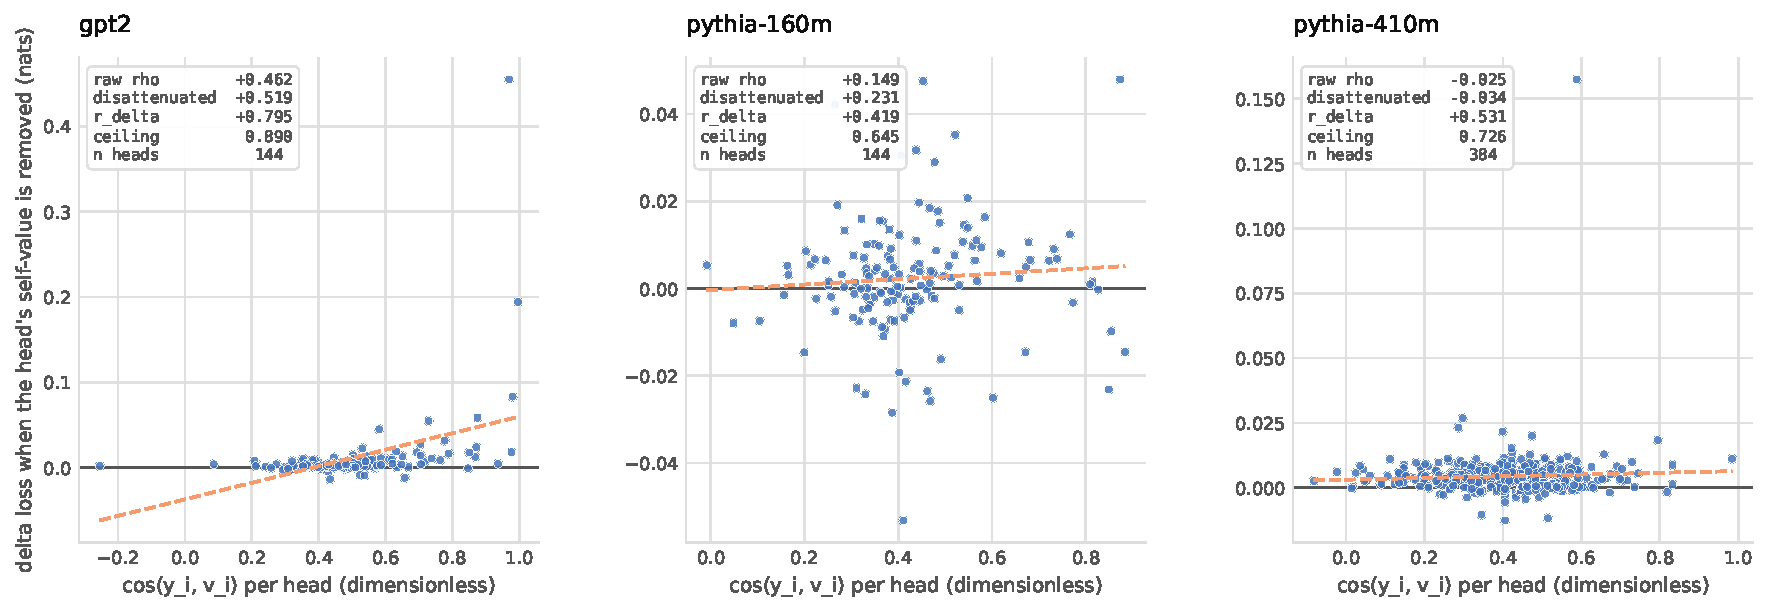
\includegraphics[width=0.98\textwidth]{figs/fig6_a2_scatter.pdf}
\caption{Structural statistic against measured behavioural effect, one panel
per model, with each panel's raw and disattenuated correlation printed on it.
The scatter is wide throughout and the fitted slope in the rightmost panel is
not distinguishable from flat. The vertical scales differ by an order of
magnitude between panels and are deliberately not shared: forcing a common
axis would compress two of the three panels into a line. The comparison across
models is therefore the correlation, not the visual spread.}
\label{fig:a2}
\end{figure*}

\begin{figure}[tb]
\centering
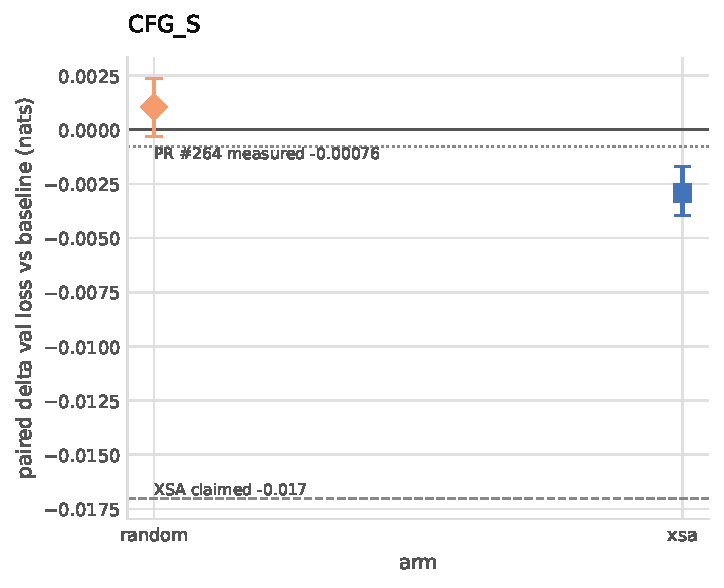
\includegraphics[width=\columnwidth]{figs/fig2_paired_delta.pdf}
\caption{Paired difference in validation loss against baseline, with $95\%$
intervals, over eight paired seeds. The \textsc{random} interval crosses zero
and the \textsc{xsa} interval does not. The two horizontal rules are external
reference points, not measurements of ours: the effect originally claimed for
this intervention ($-0.017$) and the effect an independent replication reports
($-0.00076$). Both sit outside what we measure, in opposite directions.}
\label{fig:paired}
\end{figure}

\begin{figure}[tb]
\centering
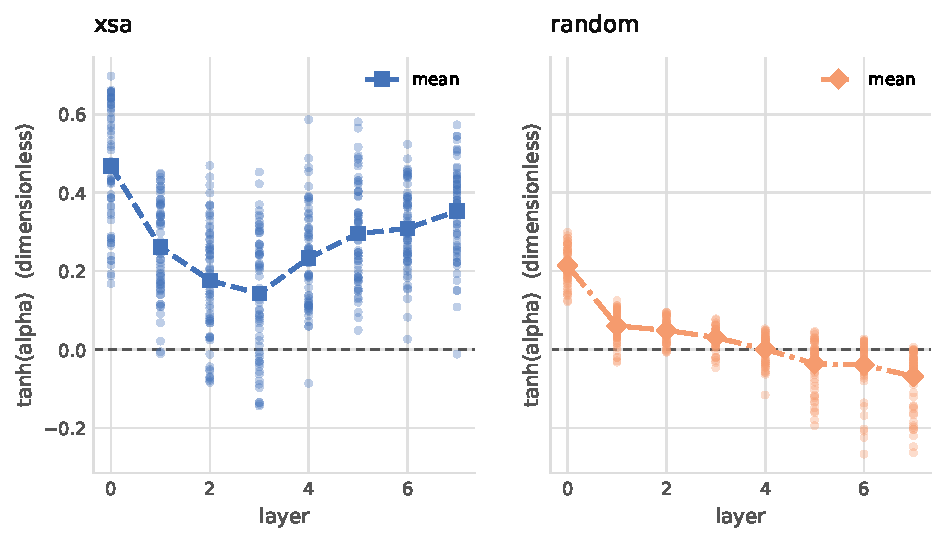
\includegraphics[width=\columnwidth]{figs/fig1_gates.pdf}
\caption{Learned gate $\tanh(\alpha)$ per layer, every head plotted, markers
at the layer mean. The \textsc{xsa} arm settles on a positive gate at every
depth, so it removes part of the self-directed component throughout training;
the \textsc{random} arm drives its gate to zero and slightly below, which is
the model switching an arbitrary rank-one removal off. The two arms are given
identical gate parameterisations, so the difference is learned rather than
imposed.}
\label{fig:gates}
\end{figure}

\begin{figure}[tb]
\centering
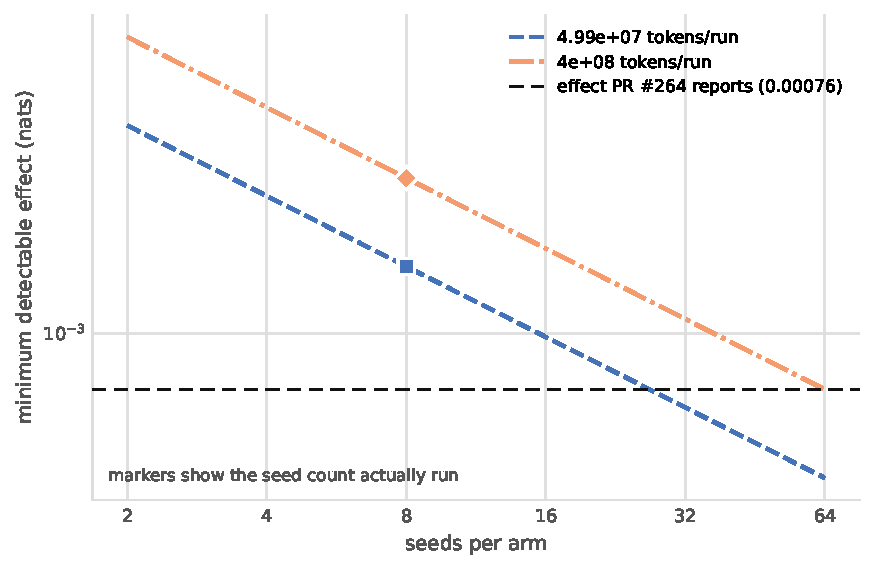
\includegraphics[width=\columnwidth]{figs/fig7_power.pdf}
\caption{Realised MDE against seeds per arm, on the two token budgets actually
run, with markers at the seed count each was run to. The dashed rule is the
effect an independent replication reports ($0.00076$); neither budget resolves
it at eight seeds, which is why we make no claim about an effect that size.}
\label{fig:power}
\end{figure}

\begin{figure}[tb]
\centering
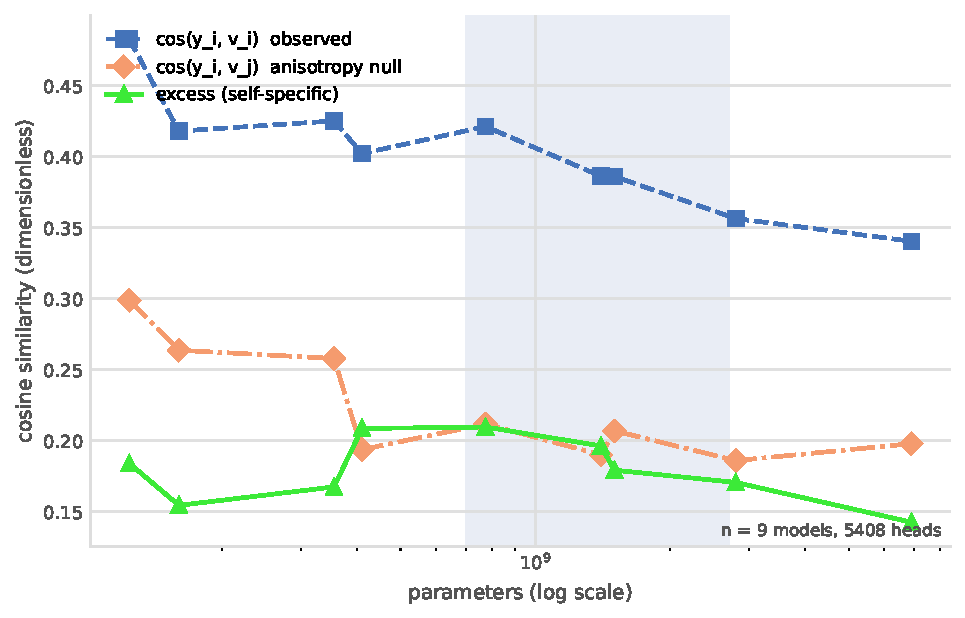
\includegraphics[width=\columnwidth]{figs/fig3_ladder.pdf}
\caption{Check~1 across the nine multi-head models in the ladder, every model
pinned by revision hash. Observed $\cos(\yv_i,\mathbf{v}_i)$, the anisotropy
null $\cos(\yv_i,\mathbf{v}_j)$, and their difference. The observed curve
declines with scale; the excess does not.}
\label{fig:ladder}
\end{figure}

\begin{figure}[tb]
\centering
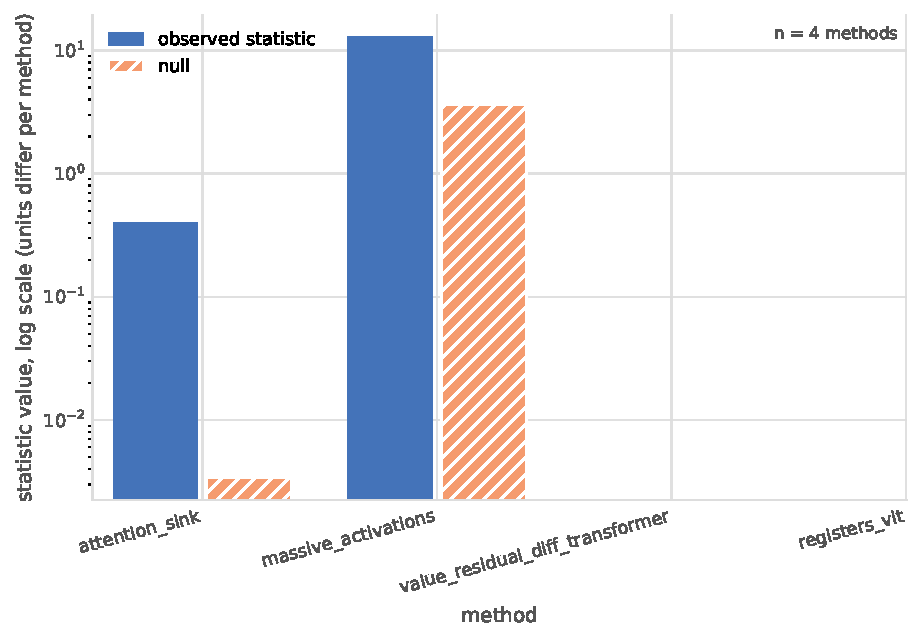
\includegraphics[width=\columnwidth]{figs/fig4_generality.pdf}
\caption{Check~1 applied to four reportedly self-specific phenomena, observed
statistic against its matched null, on a log axis because the units differ per
method. The two rightmost methods are not run---one needs a matched-capacity
control that means training two more models, the other is a vision
architecture---and are left blank rather than plotted at zero.}
\label{fig:generality}
\end{figure}

\begin{figure}[tb]
\centering
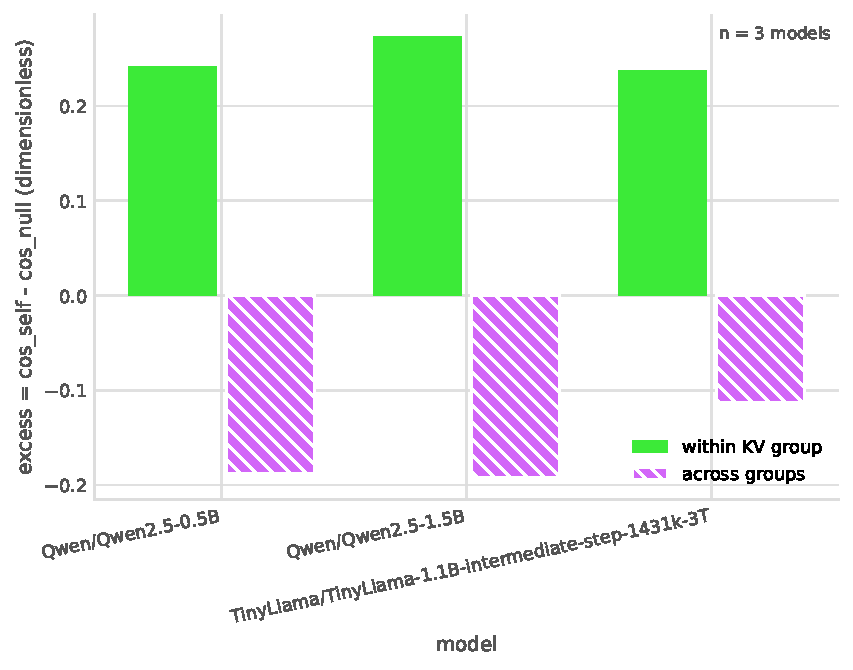
\includegraphics[width=\columnwidth]{figs/fig5_gqa.pdf}
\caption{Within-group against across-group excess for the three grouped-query
models in the ladder. The sign flip is consistent across all three. Multi-head
models are omitted rather than plotted at zero, because for them the split is
undefined, which is not the same as null.}
\label{fig:gqa}
\end{figure}


\subsection{Resolvability}

Table~\ref{tab:reliability} reports Check~0. Only GPT-2 clears the reliable
threshold; both Pythia models are attenuated, and no model is unresolvable at
the sequence length and document count used. The ceiling $\rho_{\max}$ is the
number that matters: for Pythia-160M it is $0.645$, so a raw correlation of
$0.15$ is $23\%$ of the largest value the measurement could have produced, not
$15\%$ of a perfect one.

\subsection{Structural statistic versus behavioural effect}
\label{sec:a2}

Figure~\ref{fig:a2} plots the per-head structural statistic against the
measured effect, one panel per model, and Table~\ref{tab:a2} gives the raw and
disattenuated Spearman correlations. Even in the one model where the
measurement is reliable, the disattenuated correlation for the excess statistic
is $0.313$: the structural statistic explains under ten percent of the variance
in the behavioural effect. For Pythia-410M the self-cosine statistic is
$-0.034$ after disattenuation, which is to say it carries no signal.

An earlier version of this analysis reported a substantially larger excess
correlation for Pythia-160M ($+0.487$). That figure came from reusing the
self-cosine reliability to disattenuate the excess statistic, and from pairing
a half-split statistic against a two-half effect. Corrected, it is $+0.189$,
and the claim it supported has been narrowed accordingly.

\subsection{The paired factorial}
\label{sec:paired}

Table~\ref{tab:paired} is the central result and Figure~\ref{fig:paired} shows
it as intervals. All 24 cells completed, giving eight complete paired seeds.

The pre-registered primary endpoint, \textsc{random} versus baseline, is
$+0.001056$ nats with a $95\%$ interval of $[-0.000298, +0.002390]$ and $p =
0.197$. An arbitrary rank-one removal of matched norm is therefore not
detectably harmful at this sample size, which is the precondition the design
required.

The secondary endpoint, \textsc{xsa} versus baseline, is $-0.002924$ nats with
interval $[-0.003967, -0.001709]$, $t = -4.67$, and Holm-corrected $p =
0.0023$. Removing the self-directed direction \emph{raises} loss, well outside
the interval of the matched control. The realised MDE from
Equation~\ref{eq:mde} is $0.00182$ nats for the XSA contrast and $0.00215$ for
the control contrast, so the XSA effect is roughly $1.6\times$ the smallest
effect the design could resolve while the control effect sits below it.
Figure~\ref{fig:power} places both budgets on the same power surface and shows
what the design could and could not have resolved.

This reverses the direction of the informal claim. The self-directed component
is not redundant; it is load-bearing, and the arbitrary-direction control shows
that the penalty is specific to it rather than generic to rank-one editing.

The learned gates in Figure~\ref{fig:gates} say the same thing from the other
side. Both intervened arms are free to switch their edit off by driving
$\tanh(\alpha)$ to zero, and \textsc{random} does exactly that, reaching zero
by layer four and going slightly negative below it. \textsc{xsa} does not: it
holds a positive gate at every depth, between $0.14$ and $0.47$ at the layer
mean, so it keeps removing part of the self-directed component for the whole of
training and pays for it in loss. The gate is where a redundant component
should have been cheapest to discard.

\subsection{Check 1 across the model ladder}
\label{sec:ladder}

Figure~\ref{fig:ladder} runs Check~1 over the nine multi-head models in the
ladder, covering $5408$ heads. The observed self-cosine falls from $0.44$ to
$0.34$ across three orders of magnitude of parameters, but the anisotropy null
falls alongside it, and the excess---the part that is specific to the head's
own value vector---sits between $0.14$ and $0.21$ with no monotone trend. The
raw self-cosine would have suggested a scale effect; against the null there is
none. The three grouped-query models are held out of this panel and treated
separately in Section~\ref{sec:gqa}, because for them the null partner set
straddles a shared key--value projection.

Figure~\ref{fig:generality} applies the same null to four other phenomena that
are described in the literature as self-specific. Two of the four are measured:
the attention sink survives its null almost intact ($0.403$ observed against
$0.003$ null), while massive activations do not ($12.87$ against $3.65$, so
most of the effect is present in the null). The other two are not run, and are
drawn as empty slots rather than as zeros.

\subsection{Grouped-query attention}
\label{sec:gqa}

If the self-directed read were an artefact of per-head value projections, then
sharing those projections across a group should change it. Among the twelve
models, the grouped-query models permit a within-group versus across-group
split. Three of the twelve models are grouped-query. For Qwen2.5-0.5B ($14$
query heads over $2$ key--value heads) the within-group excess is $+0.2415$ and
the across-group excess is $-0.1876$, and the other two grouped-query models
agree in sign and close in magnitude (Figure~\ref{fig:gqa}). The statistic is
positive exactly where key and value projections are shared and negative where
they are not, which is what a statistic tracking parameter sharing rather than
head identity would do. The remaining nine models are multi-head, and for those
the split does not exist; we record that explicitly rather than reporting a
value.

\section{Limitations}

\paragraph{Scale of the trained factorial.} Check~2 trains a small model at
$4.0\times10^{8}$ tokens per run. The effect is resolved at that scale, but
nothing here shows the sign or magnitude persists at the scale of the frozen
models in Checks 0 and 1. The two halves of the paper are consistent, not
continuous.

\paragraph{One statistic family.} Both structural statistics are cosine-based.
A statistic built on attention mass rather than output geometry could correlate
better with the behavioural effect, and we have not ruled that out.

\paragraph{Reliability at depth.} Only three models were carried through
Check~0, because split-half reliability at $n = 384$ heads is the most
expensive measurement in the protocol. The ladder results in
Section~\ref{sec:ladder} therefore inherit an unverified assumption that their
statistic is as reliable as the three measured models suggest.

\paragraph{The gate bounds layout, not semantics.} A reconstruction error of
$2.0\times10^{-4}$ shows that the tensors were assembled correctly. It does not
show that the direction we call $\vhat_i$ is the direction the informal claim
had in mind.

\section{Conclusion}

The claim that a head's self-directed read is redundant does not survive a
matched control. When an arbitrary rank-one removal of the same norm is run as
the pre-registered primary arm, it is indistinguishable from baseline, while
the self-directed removal costs $0.0029$ nats at $p = 0.0023$. The structural
statistic that motivated the claim, meanwhile, is reliable in one of three
models and predicts the behavioural effect weakly even there.

The wider point is procedural. The result that would have been reported without
Check~0 is a near-zero correlation read as decoupling; without Check~2's
control arm it is a small loss increase read as noise. Both readings are wrong,
and both are available from the same data. Interventional claims about internal
structure need their nulls stated before the number is interpreted.

\section*{Reproducibility Statement}

Every number in this paper is regenerated from committed result files by a
single script, and a test in continuous integration fails if any rendered
number disagrees with its source row. All twelve models are pinned by revision
hash. The token budget, seed list, and arm definitions are given in
Section~\ref{sec:check2} and are the exact command-line arguments used. The
underpowered $5\times10^{7}$ pilot is retained separately and labelled, so the
primary and pilot results cannot be confused. The reconstruction gate threshold
and the four broken layouts used to derive it are reproduced by a test.

\section*{Ethics Statement}

This work analyses the internal structure of publicly released pretrained
language models and trains small models from scratch on public text. It
introduces no new data collection, no human subjects, and no deployed system.
The main foreseeable misuse is citation of the negative result as licence to
prune attention components in production without running the matched control
that produced it; Section~\ref{sec:check2} states the control explicitly for
that reason.

\bibliographystyle{plainnat}
\bibliography{references}

\appendix

\section{Arm Definitions}
\label{app:arms}

\textsc{baseline} applies no intervention. \textsc{xsa} applies
Equation~\ref{eq:xsa} with the gate held open. \textsc{random} applies
Equation~\ref{eq:xsa} with $\vhat_i$ replaced by a fresh uniform unit vector at
each position. \textsc{meanval} replaces $\vhat_i$ with the normalised
batch-mean value vector, and \textsc{diagmask} sets the attention diagonal to
$-\infty$ before the softmax so the row renormalises over the remaining keys.
Only the first three arms appear in the trained factorial; the last two are
frozen-model anchors.

\section{Budget Ledger}
\label{app:budget}

The ledger records a row after each seed block completes, so the accounting
unit is a complete paired seed rather than a cell. The billed quantity is pod
uptime: training cells run inside that clock, and adding cell hours to uptime
would count the same minutes twice. An earlier projection that made exactly
that error forecast \$18.16 against a realised \$13.41 at the same point in the
run.

\section{Deviations from the Pre-Registration}
\label{app:deviations}

Two deviations are material. First, the sequence length for Checks 0 and 1 was
fixed at $128$ tokens after an initial run allowed it to drift with document
count ($142$ tokens at $24$ documents, $137$ at $64$), which matters because
Check~1's null partner set grows with length. Second, the disattenuation
procedure was corrected as described in Section~\ref{sec:a2}, which lowered the
Pythia-160M excess correlation from $+0.487$ to $+0.189$. Both original runs
are retained.

\end{document}
